\documentclass[conference]{IEEEtran}
% \IEEEoverridecommandlockouts
% The preceding line is only needed to identify funding in the first footnote. If that is unneeded, please comment it out.
\usepackage{cite}
\usepackage{amsmath,amssymb,amsfonts}
\usepackage{algorithmic}
\usepackage{graphicx}
\usepackage{textcomp}
\usepackage{xcolor}
\def\BibTeX{{\rm B\kern-.05em{\sc i\kern-.025em b}\kern-.08em
    T\kern-.1667em\lower.7ex\hbox{E}\kern-.125emX}}
\begin{document}

\title{Overview of Chaos Engineering and Chaos Mesh}

\author{\IEEEauthorblockN{Gábor Major}
\IEEEauthorblockA{\textit{Department of Computing} \\
\textit{South East Technological University}\\
Carlow, Ireland \\
C00271548@setu.ie}
}

\maketitle

\begin{abstract}
This document is an explanation on what Chaos Engineering is, and the type of testing it is useful for, creating resilient Kubernetes systems, and the advantages and disadvantages it has is also discussed. Afterwards a few technologies that are used for Chaos Engineering are mentioned with one of them, Chaos Mesh, explored in further detail at its usage and features.
\end{abstract}

\begin{IEEEkeywords}
testing, Kubernetes, distributed, experiments
\end{IEEEkeywords}

\section{Introduction}
This report has been written for 4\textsuperscript{th} year Software Development Cloud Data Centres module. This report is the end of year project on a chosen cloud computing topic. The focus of this report is on the Chaos Engineering technology, going over the definition and motivation for it as a tool, and an associated program Chaos Mesh, which is a specific tool for testing Kubernetes systems.

\section{Chaos Engineering}
\subsection{Definition}

Chaos engineering is defined as ``... the practice of intentionally introducing faults into a system in order to test its resilience and ensure applications and engineering teams are able to withstand turbulent and unexpected events.'' by the Cloud Native Computing Foundation. \cite{b1}

It is a testing method where various parts of a system while running in either a production or pre-production environment are turned off or faults are introduced into different components, to test the live resiliency of the various subsections of the whole system.

\subsection{Motivation}

The reason for chaos engineering existing is to help with testing systems that have been deployed and have many different parts working together as one. While traditional software development has black box testing for the methods and functions of a program and white box testing for the program as a whole, the next step is to test the many programs working together.

The purpose of chaos engineering is not to outright make a bulletproof system that is able to withstand a large amount of failures in the system, but instead it is focused on improving the response and recovery process of an organisation or system, and testing realistic stress scenarios. For example, it would not be very helpful to test the system where all the back end servers are simulated as failed, and instead test a more likely scenario like drastically increasing traffic of the service, putting heavy load on the system, giving better feedback on the system's resiliency.

Chaos engineering also allows not just a one-off testing of a system, or a scheduled period of running tests, but also the execution of tests by integrating them into the continuos integration and continuos delivery pipelines. \cite{b2} \\
This allows projects to have a greater amount of automatic tests running every time a change is made to any of the components of a system. They may not be able to eliminate all problems on deployment, however they filter out common issues such as no backups for a system upon updating the configuration files.

\subsection{History}

The concept of chaos engineering is not new, in 1983 while working on software for the first Apple Macintosh computer a program was created by Steve Capps called ``Monkey'' to test the user interface of the programs, by generating random high speed user input.\\
Many other companies use some sort of chaos engineering, the most notable being Netflix which regularly conducts failure tests on their production environments. They have developed their own tool called ``Chaos Monkey'' which when ran disables parts of the system to test their resilience. This has changed the mentality of teams at Netflix to take into account that any of their programs may turn offline, which makes sure they always have backup programs. \cite{b3}

\subsection{Types of Experiments}

Chaos engineering tests are also known as chaos engineering experiments. There are many different types of experiments, but the four main categories are as follows:
\begin{itemize}
	\item Latency injection: Where network connections between programs are stopped or delays are simulated.
	\item Fault injection: Where errors are introduced into the system in which one or many components may shut down or malfunction. Errors include software and hardware issues.
	\item Load generation: Where the system is stress tested using a large amount of traffic beyond the normal levels of operating capacity.
	\item Canary testing: Where new features are introduced to a small group of users to allow any errors or bugs to occur for only that select few. \cite{b2}
\end{itemize}

\subsection{Advantages and Disadvantages}

As any other type of technology chaos engineering has some advantages and disadvantages to its use. Overall it is a positive tool to test the resilience and availability of a system offering the following advantages:
\begin{itemize}
	\item Allows for better customer satisfaction as the system used by them becomes more resilient and fault-tolerant.
	\item Improves the security of the system not just by testing for denial of service attempts, but also by speeding up the discovering of vulnerabilities and the patching of bugs.
	\item Minimise the downtime caused by any disruptions to the system. As a result of testing many different scenarios of faults people will be more informed of the issues that may occur and have response or recovery plans in place for quickly remedying faults.
	\item Increases the ability to upgrade, extend and maintain the system. Experiments allow people to gauge what resources are used, and how the system functions in low and high times of use. These experiments also encourage documenting the system's quirks and edge cases for other people who may later work on the system.
\end{itemize}
There are however a few disadvantages to using chaos engineering as a tool for testing the resilience of systems:
\begin{itemize}
	\item Has a high upfront cost for a large system. Running chaos experiments on a large and previously untested programs will cause a lot of faults to be discovered at the start of testing which may not bring back noticeable returns straight away. 
	\item Has a higher maintenance cost with not just the constant executing of experiments but also the running of redundant programs to deal with the potential issues.
	\item May require a shift in mentality for people working on the system and potential rewrite of some programs.
	\item Incorrectly running experiments on production environments may lead to unwanted downtime for customers if new unaccounted faults are found. \cite{b2}
\end{itemize}

\subsection{Programs}

There are many programs and technologies available to try out and work with chaos experiments. As previously mentioned ``Chaos Monkey'' and also ``Simian Army'' are tools used by Netflix, but other simple and more complex programs are open to be used in any software projects. Some programs are as follows:
\begin{itemize}
	\item Litmus
	\item Chaos Toolkit
	\item Chaos Blade
	\item krkn \cite{b1}
\end{itemize}
A smaller interesting project ``chaoskube'' is a simple application to run chaos experiments. It allows killing pods in any namespace at regular intervals. It also has filters and other settings in place to limit the amount of damage the program is able to cause. \cite{b4} \\
A bigger and more mature technology is ``Chaos Mesh''. This will be explored in the following sections of the document.


\section{Chaos Mesh}
\subsection{Overview}

Chaos Mesh is described as a cloud-native Chaos Engineering platform. It is able to run anywhere where Kubernetes is deployed. Using the platform, it is possible to create different types of fault scenarios simulations. Chaos Mesh is a powerful tool for orchestrating systems testing. It is however not a terminal only program as a convenient Web UI (User Interface) is available to support the operations of testing and experimenting.\\
Some of the core strengths of Chaos Mesh include:
\begin{itemize}
	\item Stable History
	\item Used by Numerous Companies
	\item Easy to Use System
	\item Cloud Native
	\item Various Simulations
	\item Flexible Experimentations
	\item High Security
	\item Active Community
	\item Easily Scalable
\end{itemize}

Chaos Mesh is made up of three core components which communicate together to achieve the functionality set out by the program:
\begin{itemize}
	\item Chaos Dashboard: This is the Web UI that is used for creating, running and observing Chaos experiments. The usage of this is not necessary as the program can use YAML (YAML Ain't Markup Language) files for running the experiments
	\item Chaos Controller Manager: This is the core component of Chaos Mesh as it is responsible for all logical operations such as scheduling and managing the experiments. As Chaos Mesh was built on Kubernetes CRD (Custom Resource Definition) the Chaos Controller Manager contains many different CRD controllers to perform its task, such as Workflow Controller and Scheduler Controller.
	\item Chaos Daemon: Responsible for the execution of controllers' commands. The Chaos Daemon is run with privileged permissions by default, and is allowed to interfere with network devices, file systems, and kernels to run the experiments.
\end{itemize}

Following is a diagram showing on how the different components of Chaos Mesh are situated in a Kubernetes environment. From the top users interact with the Kubernetes API (Application Programming Interface) Server either through the dashboard or not. The Chaos Controller Manager then takes these commands and runs them. Finally, the Chaos Daemon is inside the node where fault injection takes place to disrupt and test the system.

\begin{figure*}
	\centering
	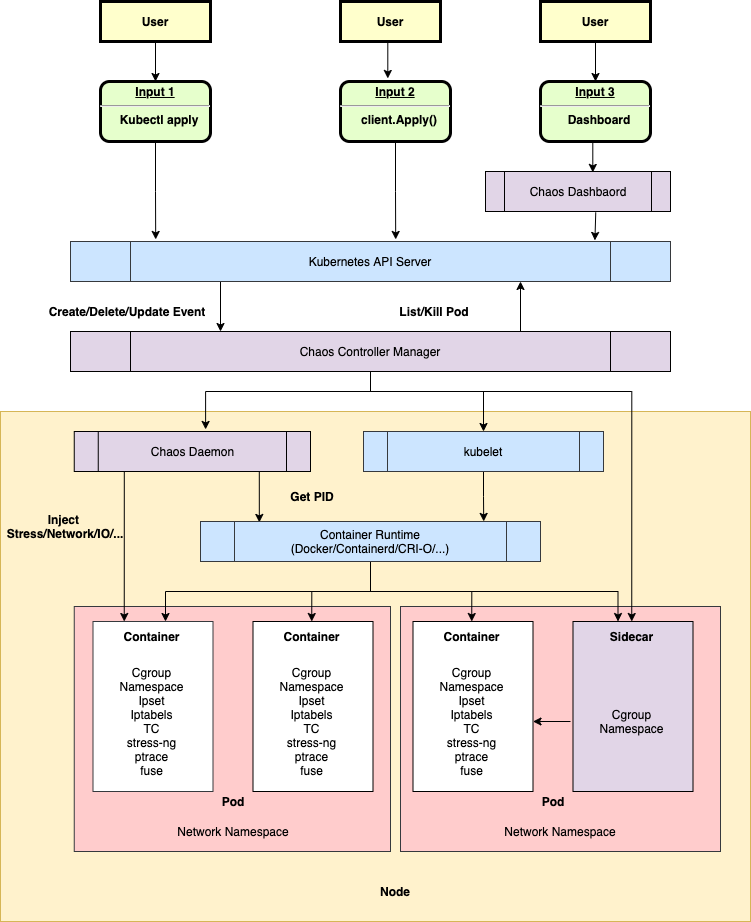
\includegraphics[width=0.71\linewidth]{chaos_mesh_diagram}
	\caption{Architecture diagram of Chaos Mesh.}
	\label{fig:chaosmeshdiagram}
\end{figure*}


\subsection{Features}

There are four features that define Chaos Mesh, fault injection, Chaos workflows, visualised operations and security guarantees.

\paragraph{Fault Injection}
Fault injections are the basis of Chaos experiments. They come in three different categories giving a wide range of potential problems that could happen in a distributed system.\\
Basic resource faults are the first group which contain simulations affecting the Pods' availabilities, manipulating network conditions, DNS and HTTP disruptions, CPU, memory I/O (Input/Output), time and kernel failures.\\
Platform faults are also available for simulating AWS (Amazon Web Services), Azure, and GCP (Google Cloud Platform) failures and node restarts.\\
Finally, application faults are the third type of fault injection, which simulates JVM (Java Virtual Machine) failures.

The above fault injections can be run as Chaos experiments on either Kubernetes or there is also an option to run Chaos experiments on physical machines using the Chaosd tool in Chaos Mesh. This tool is a bit more limited in faults it can create, however this tool runs on the physical machine which may cause multiple different pods to become unreliable.

\paragraph{Chaos Workflows}
Chaos workflows are a step up from the Chaos experiments, they allow the set-up of multiple Chaos experiments bundled together to perform a specific testing workflow. Using Chaos workflows it is possible to orchestrate serial or parallel Chaos experiments, check the status and results of experiments and applications, and using YAML files or the Web UI to manage the Chaos workflows.

\paragraph{Visualised Operations}
The Chaos Dashboard allows for an easy Web UI overview of statistics, and the quick creation and management of Chaos experiments.

\begin{figure*}
	\centering
	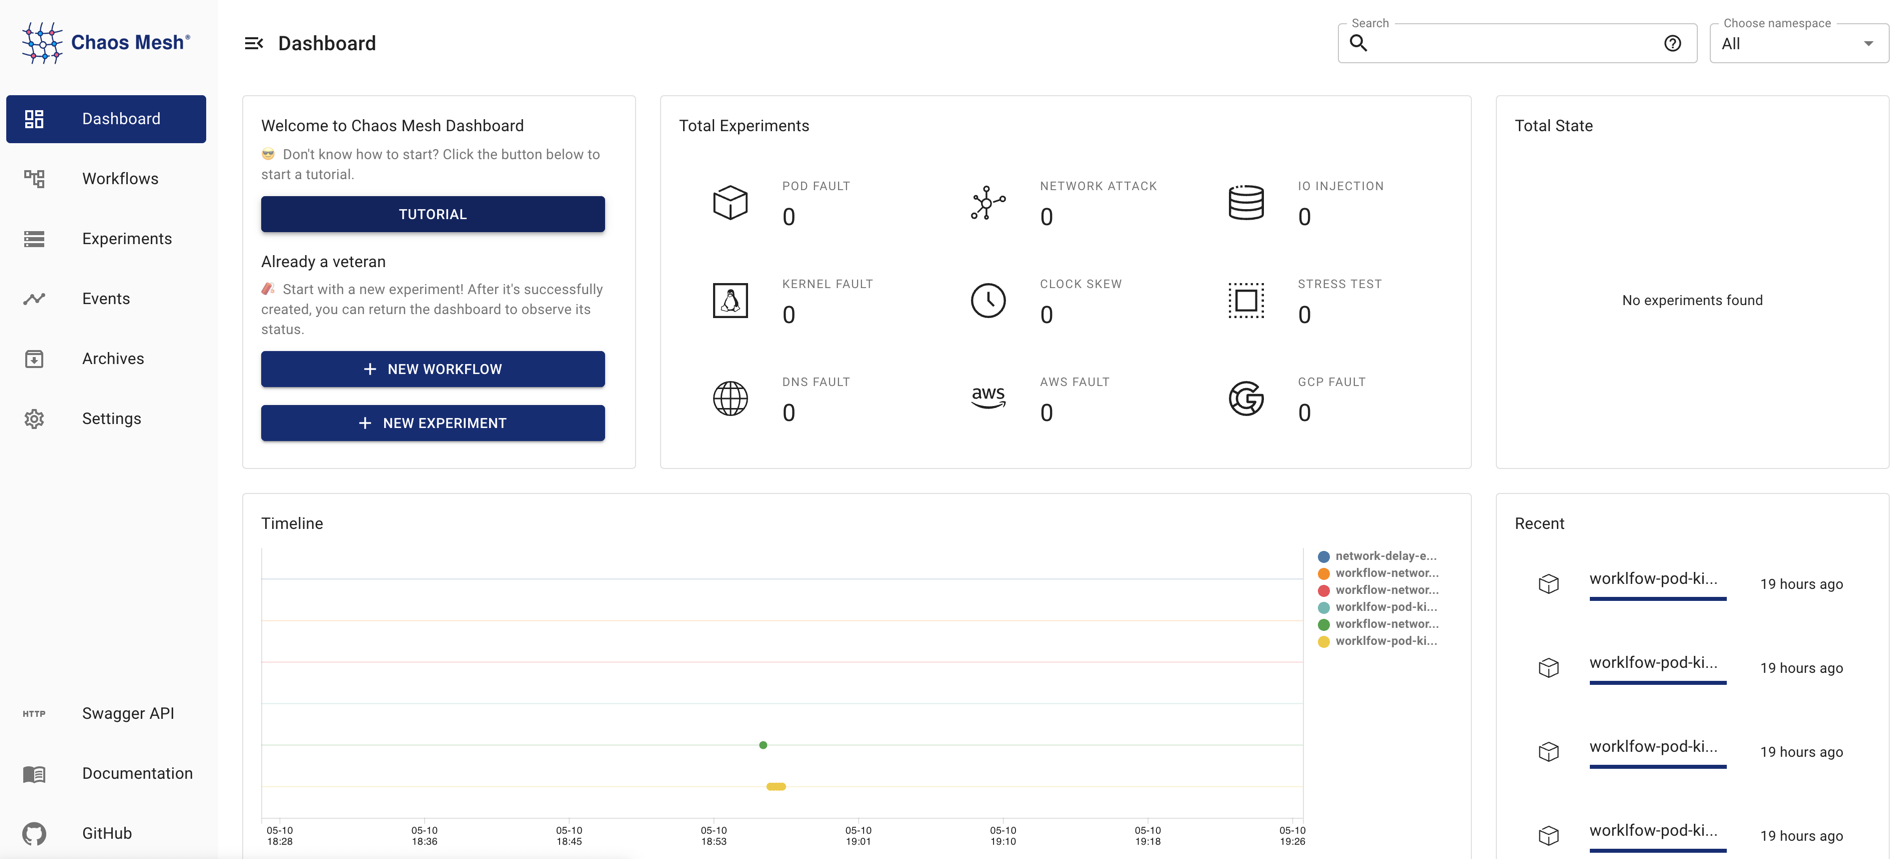
\includegraphics[width=0.8\linewidth]{chaos_mesh_dashboard}
	\caption{Chaos Mesh dashboard.}
	\label{fig:chaosmeshdashboard}
\end{figure*}


\paragraph{Security Guarantees}
Chaos Mesh allows for the creation of different roles for differing levels of Chaos experiment permissions. Furthermore, namespaces can be specified for the experiments limiting their abilities.

Different user accounts may also be registered for creating permissions such as view only accounts, or accounts that have access to only specific types of Chaos experiments or workflows.


\subsection{Running Chaos Experiments}

Chaos experiments can be run either individually or multiple together in a workflow. When creating Chaos experiments various options may be configured such as the scope it is allowed to operate on, the scheduling rules such as the run time for the experiment and when to run it.\\
Similarly, in Chaos workflows you can set the types of Chaos experiments to run, when to run them or how to run them i.e. in serial or parallel.

\begin{figure}
	\centering
	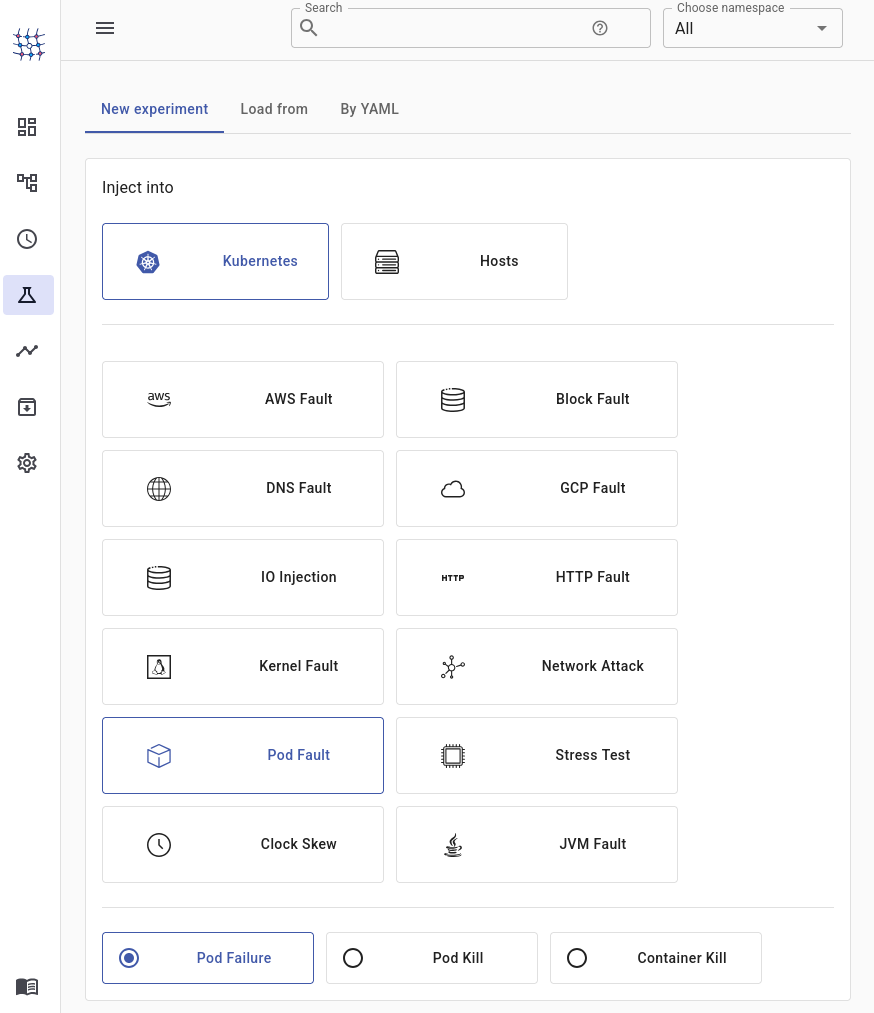
\includegraphics[width=0.8\linewidth]{chaos_mesh_new_experiment_kubernetes}
	\caption{Web UI for creating Kubernetes experiment.}
	\label{fig:chaosmeshnewexperimentkubernetes}
\end{figure}

\begin{figure}
	\centering
	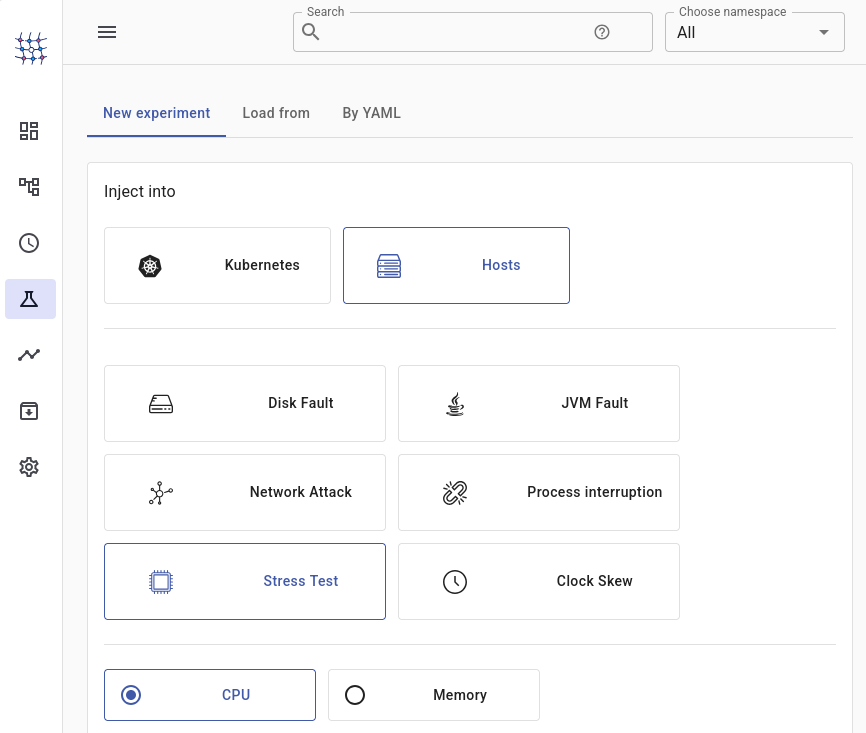
\includegraphics[width=0.7\linewidth]{chaos_mesh_new_experiment_hosts}
	\caption{Web UI for creating host experiment.}
	\label{fig:chaosmeshnewexperimenthosts}
\end{figure}

\subsection{Integration}

Chaos Mesh has the capabilities to be integrated into other workflows such as GitHub Actions, which is a continuous integration and continuous deployment feature created by GitHub. This allows the building and testing of code using the Chaos Mesh toolset every time there is an update to the code on GitHub. \cite{b5}

\subsection{Testing Single Experiment}

First Minikube was set up, along with the Hello Minikube pod and Chaos Mesh.

\begin{figure*}
	\centering
	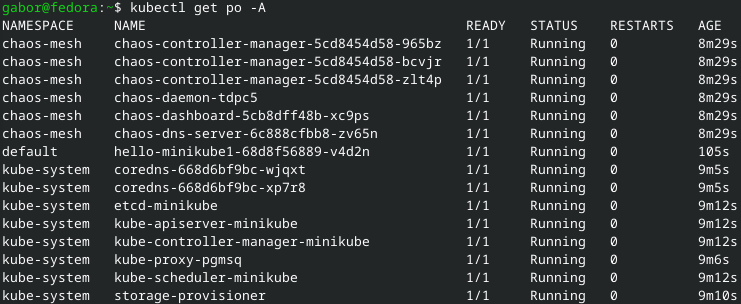
\includegraphics[width=0.7\linewidth]{hello_minikube_running}
	\caption{Hello Minikube node running.}
	\label{fig:hellominikuberunning}
\end{figure*}

Next the Hello Minikube website was accessed from the web browser showing a success in connecting.

\begin{figure}
	\centering
	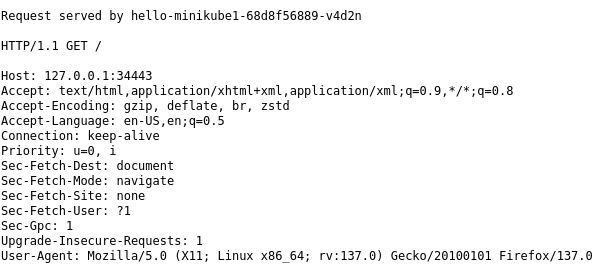
\includegraphics[width=0.8\linewidth]{hello_minikube_result}
	\caption{Success on accessing.}
	\label{fig:hellominikuberesult}
\end{figure}

Then the following Chaos experiment was run using the YAML file.

\begin{figure}
	\centering
	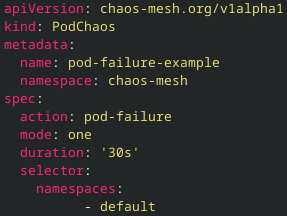
\includegraphics[width=0.6\linewidth]{pod_failure}
	\caption{Contents of pod-failure.yaml.}
	\label{fig:podfailure}
\end{figure}


It was applied to the running Hello Minikube pod, resulting in the web service being unavailable for 30 seconds.

\begin{figure}
	\centering
	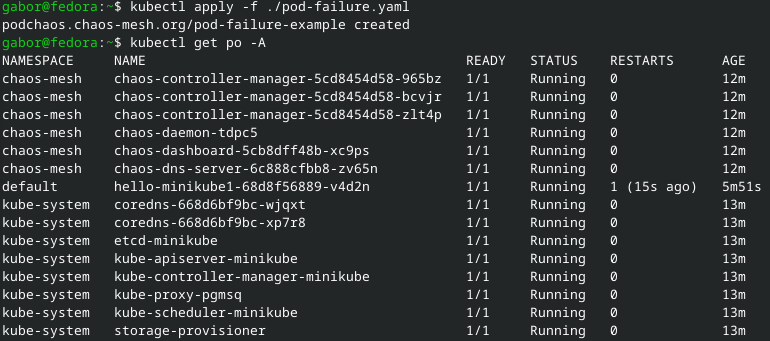
\includegraphics[width=1\linewidth]{hello_minikube_restarted}
	\caption{Apply experiment and pod stopped.}
	\label{fig:hellominikuberestarted}
\end{figure}

\section{Conclusion}

Chaos Engineering is a valuable tool to have available for testing the different systems that are deployed to Kubernetes. It may not give bulletproof results against all system faults, however it does allow the speeding up of and more importantly the automating of testing. If any company or organisation is working with Kubernetes then there should definitely be at least some basic type of testing tool implemented. As cloud programs can grow to become quite big systems, it is essential to implement good programming and testing practices.

\begin{thebibliography}{00}
\bibitem{b1} Cloud Native Computing Foundation,  ``Chaos Engineering'',  2024,  https://landscape.cncf.io/guide\#observability-and-analysis--chaos-engineering

\bibitem{b2} IBM, ``What is chaos engineering?'', 3 August 2023,  https://www.ibm.com/think/topics/chaos-engineering

\bibitem{b3} Wikipedia, ``Chaos engineering'', 27 September 2024, https://en.wikipedia.org/wiki/Chaos\_engineering

\bibitem{b4} chaoskube, ``chaoskube GitHub repository'', 29 April 2025,
https://github.com/linki/chaoskube

\bibitem{b5} Chaos Mesh, ``Chaos Mesh Documentation'', 1 May 2025, https://chaos-mesh.org/docs/

\end{thebibliography}

\end{document}
